\documentclass[../sotsu.tex]{subfiles}

\begin{document}


\section{商空間とテンソル積}

この節では,
複数の量子状態を扱ううえで必須であるテンソル積を取り扱う\footnote{
    どういうわけか,%
    $\psi (x, y) = \varphi_1 (x) \varphi_2(y)$に対して%
    $\varphi_1$のみに作用する演算子$D = D(x)$を作用させると%
    $D(x) \psi(x, y) = (D \varphi_1 (x)) \varphi_2 (y)$となることから類推して,
    $\ket{\psi} = \ket{\varphi_1} \ket{\varphi_2}$に対して%
    $\varphi_1$のみに作用する演算子$\hat{D}_1$を作用させると%
    $\hat{D}_1 \ket{\psi} = (\hat{D}_1 \ket{\varphi_1}) \ket{\varphi_2}$である%
    という定義が\ruby{罷}{まか}り通っているようである.
    しかし,$\ket{\varphi_1}, \ket{\varphi_2}$をベクトルと考えたとき,
    ベクトルを横に並べた$\ket{\varphi_1} \ket{\varphi_2}$とはどういうものなのか,
    さらに左側のベクトルにだけ作用する演算子=行列とはどういうものなのか,
    これではまったく意味不明である.
}.


\subsection{商空間}

ベクトル空間の\refdfn[商集合]{dfn:quotient-set}に対応する.

\begin{definition}
    \label{dfn:quotient-space}
    $V$を$\symbb{K}$上のベクトル空間,$W$を$V$の\refdfn[部分ベクトル空間]{dfn:vector-subspace}とする.
    $V$上の\refdfn-[同値関係]{dfn:equivalence-relation}$\sim$を
    \begin{equation}
        𝒙 \sim 𝒚
            \iff  𝒙 - 𝒚 \in W
    \end{equation}
    と定義し,
    $\sim$による同値類を$\eqclass{𝒙}$とかくことにする.
    商集合を$V/W$とかき,\word{商空間}とよぶ.
\end{definition}

\begin{proposition}
    商空間$V/W$は次のような和とスカラー倍のもとでベクトル空間をなす.
    \begin{subequations}
    \begin{align}
        \eqclass{𝒙} \mathbin{\bar{+}} \eqclass{𝒚} &\coloneq \eqclass{𝒙 + 𝒚}  \\
        c \mathbin{\bar{\scaprod}} \eqclass{𝒙} &\coloneq \eqclass{c𝒙}
    \end{align}
    \end{subequations}
\end{proposition}

\begin{proof}
    $\mathbin{\bar{+}}$と$\mathbin{\bar{\scaprod}}$がwell-definedであることを示せば十分だろう.
    
    まず$𝒙 \sim 𝒙'$,$𝒚 \sim 𝒚'$とする.
    このとき$\symbf{w} \coloneq 𝒙 + 𝒚 \in W$,
    $\symbf{w}' \coloneq 𝒙 + 𝒚 \in W$であるから,
    $\symbf{w} - \symbf{w}' \in W$である.
    つまり$(𝒙 + 𝒚) - (𝒙' + 𝒚') \in W$,
    だから$𝒙 + 𝒚 \sim 𝒙' + 𝒚'$である.

    次に,$𝒙 - 𝒙' \in W$だから,
    $c𝒙 - c𝒙' = c(𝒙 - 𝒚) \in W$.
    よって,$c𝒙 \sim c𝒙'$である.
\end{proof}


\subsection{テンソル積}
\label{sec:tensor-product-of-vector}

$V, W$を$\symbb{K}$上のベクトル空間とする.
$𝒙, 𝒙' \in V$,$𝒚, 𝒚' \in W$,$c \in \symbb{K}$について,
\begin{subequations}
\label{eq:bilinear-map}
\begin{align}
    (𝒙 + 𝒙^{\mathrlap{\prime}}, \  𝒚) &= (𝒙, 𝒚) + (𝒙^{\mathrlap{\prime}}, 𝒚)
    &
    (c𝒙, 𝒚) &= c(𝒙, 𝒚)
    \\
    (𝒙, \  𝒚 + \symbf{y}') &= (𝒙, 𝒚) + (𝒙, 𝒚')
    &
    (𝒙, c𝒚) &= c(𝒙, 𝒚)
\end{align}
\end{subequations}
が成り立つような$(𝒙, 𝒚)$を\word{テンソル積}\index{てんそるせき@テンソル積}という.
$(𝒙, 𝒚)$の全体もまた,ベクトル空間をなすので,
この空間を$V \otimes W$とかく.
また$(𝒙, 𝒚) \eqcolon 𝒙 \otimes 𝒚$とかく.

なお,\cref{eq:bilinear-map}のような条件を満たす写像$(\bigdot, \bigdot)$を\word{双線形写像}という.

定義を見てもわかりづらいので,
具体例でみてみよう.
$V = V' = W = W' = \symbb{R}^2$とする.
2つのベクトルのテンソル積は
\begin{equation}
    \label{eq:tensor-product-of-2-vector}
    \begin{pmatrix}
        a \\ b
    \end{pmatrix}
    \otimes
    \begin{pmatrix}
        c \\ d
    \end{pmatrix}
    \coloneq
    \begin{pmatrix}
        a 
        \begin{pmatrix}
            c \\ d
        \end{pmatrix}
        \\
        b
        \begin{pmatrix}
            c \\ d
        \end{pmatrix}
    \end{pmatrix}
    =
    \begin{pmatrix}
        ac \\ ad \\ bc \\ bd
    \end{pmatrix}
\end{equation}
とかける.
もちろん$\symbb{R}^2 \otimes \symbb{R}^2$の次元は$2 \times 2 = 4$であり,
その基底は
\begin{equation}
    \label{eq:basis-of-tensor-product-of-2-vector}
    \begin{split}
        \begin{pmatrix}
            1  \\  0
        \end{pmatrix}
        \otimes
        \begin{pmatrix}
            1  \\  0
        \end{pmatrix}
        =
        \begin{pmatrix}
            1  \\  0  \\  0  \\  0
        \end{pmatrix}
        ,
        \quad
        \begin{pmatrix}
            1  \\  0
        \end{pmatrix}
        \otimes
        \begin{pmatrix}
            0  \\  1
        \end{pmatrix}
        =
        \begin{pmatrix}
            0  \\  1  \\  0  \\  0
        \end{pmatrix}
        ,
        \\
        \begin{pmatrix}
            0  \\  1
        \end{pmatrix}
        \otimes
        \begin{pmatrix}
            1  \\  0
        \end{pmatrix}
        =
        \begin{pmatrix}
            0  \\  0  \\  1  \\  0
        \end{pmatrix}
        ,
        \quad
        \begin{pmatrix}
            0  \\  1
        \end{pmatrix}
        \otimes
        \begin{pmatrix}
            0  \\  1
        \end{pmatrix}
        =
        \begin{pmatrix}
            0  \\  0  \\  0  \\  1
        \end{pmatrix}
        .
    \end{split}
\end{equation}
である.
すなわち,
$\symbb{R}^2 \otimes \symbb{R}^2 = \symbb{R}^4$と考えられる.

\cref{eq:basis-of-tensor-product-of-2-vector}の線形結合でかけるベクトルはすべて$\symbb{R}^2 \otimes \symbb{R}^2$に属する.
ところが,そのようなベクトルが\cref{eq:tensor-product-of-2-vector}の形で書けるとは限らない.
例えば\(
    \tp{(1 \; 0)} \otimes \tp{(1 \; 0)} + \tp{(0 \; 1)} \otimes \tp{(0 \; 1)}
    =
    \tp{(1 \; 0 \; 0 \; 1)} \in \symbb{R}^2 \otimes \symbb{R}^2
\)は2つのベクトルのテンソル積としてかけない\footnote{
    $\tp{(1 \; 0 \; 0 \; 1)}$が\cref{eq:tensor-product-of-2-vector}で表せたとする.
    第2成分より$ad = 0$だから,$a=0$または$d=0$.
    $a=0$であれば,第1成分($ac = 1$)と矛盾.
    $d=0$とすると,第4成分($bd = 1$)と矛盾.
}.
この事実が量子エンタングル状態を引き起こす.

一方,\( V = V' = W = W' = \text{$2 \times 2$-行列全体の集合} \)とする.
このとき,テンソル積は
\begin{equation}
    \label{eq:tensor-product-of-2-matrix}
    \begin{pmatrix}
        a  & b  \\ c  & d 
    \end{pmatrix}
    \otimes 
    \begin{pmatrix}
        \alpha & \beta \\ \gamma & \delta
    \end{pmatrix}
    =
    \begin{pmatrix}
        a
        \begin{pmatrix}
            \alpha & \beta \\ \gamma & \delta
        \end{pmatrix}
        &
        b
        \begin{pmatrix}
            \alpha & \beta \\ \gamma & \delta
        \end{pmatrix}
        \\
        c
        \begin{pmatrix}
            \alpha & \beta \\ \gamma & \delta
        \end{pmatrix}
        &
        d
        \begin{pmatrix}
            \alpha & \beta \\ \gamma & \delta
        \end{pmatrix}
    \end{pmatrix}
    =
    \begin{pmatrix}
        a \alpha  &  a \beta   &  b \alpha  &  b \beta   \\
        a \gamma  &  a \delta  &  b \gamma  &  b \delta  \\
        c \alpha  &  c \beta   &  d \alpha  &  d \beta   \\
        c \gamma  &  c \delta  &  d \gamma  &  d \delta  
    \end{pmatrix}
\end{equation}
とかける.
このような定義の下で,
行列$A, B$とベクトル$\symbf{x}, \symbf{y}$について
\begin{equation*}
    (A \otimes B) (\symbf{x} \otimes \symbf{y}) 
        = (A \symbf{x}) \otimes (B \symbf{y})
\end{equation*}
が成り立つことも容易に示される(\cref{sec:tensor-product-of-linear-map}も参照).

3つ以上のテンソル積についても,帰納的に定義される.
すなわち,$\symbf{x}, \symbf{y}, \symbf{z} \in \symbb{R}^2$のテンソル積は,
\begin{equation*}
    \symbf{x} \otimes \symbf{y} \otimes \symbf{z}
    \coloneq 
    \symbf{x} \otimes (\symbf{y} \otimes \symbf{z})
\end{equation*}
である.
$\symbf{x} \otimes (\symbf{y} \otimes \symbf{z}) = (\symbf{x} \otimes \symbf{y}) \otimes \symbf{z}$であることは容易に示される.
$\symbb{R}^2 \otimes \symbb{R}^2 \otimes \symbb{R}^2 = \symbb{R}^8$であり,
これを$(\symbb{R}^2)^{\otimes 3}$とも書く.


\begin{proposition}
    \label{thm:tensor-product-bilinear}
    $V, W$を\refdfn-[$\symbb{K}$]{dfn:field}上のベクトル空間,
    $\symbf{x}, \symbf{x}' \in V, \  \symbf{y}, \symbf{y}' \in V, \  c \in \symbb{K}$について,
    以下が成り立つ.
    \begin{enumerate}
        \item $(\symbf{x} + \symbf{x}') \otimes \symbf{y} = (\symbf{x} \otimes \symbf{y}) + (\symbf{x}' \otimes \symbf{y})$
        \item $\symbf{x} \otimes (\symbf{y} + \symbf{y}') = (\symbf{x} \otimes \symbf{y}) + (\symbf{x} \otimes \symbf{y}')$
        \item $(c \symbf{x}) \otimes \symbf{y} = c (\symbf{x} \otimes \symbf{y}) = \symbf{x} \otimes (c \symbf{y})$
    \end{enumerate}
\end{proposition}

むしろ,\cref{thm:tensor-product-bilinear}が成り立つようにテンソル積を定めたのであった.




\subsubsection{テンソル積の構成}

\begin{definition}
    \label{dfn:tensor-product}
    線形汎関数$h \colon V \times W \to \symbb{K}$の中で,
    $h(\symbf{x}, \symbf{y}) \neq 0$となる$(\symbf{x}, \symbf{y}) \in V \times W$の数が有限個であるもの全体の集合を$L$と書くことにする.
    $L$の元であって,
    \begin{equation*}
        e_{\symbf{x}, \symbf{y}} (\symbf{x}', \symbf{y}') = 
        \begin{cases}
            1  &  \text{if } (\symbf{x}, \symbf{y}) = (\symbf{x}', \symbf{y}')  \\
            0  &  \text{if } (\symbf{x}, \symbf{y}) \neq (\symbf{x}', \symbf{y}')
        \end{cases}
    \end{equation*}
    となるものを考えよう.
    $\sequ{e_{\symbf{x}, \symbf{y}}}[\symbf{x} \in V, \, \symbf{y} \in W]$は$L$の基底になっている\footnote{
        $L$の定義から$h(\symbf{x}, \symbf{y}) \neq 0$となる$(\symbf{x}, \symbf{y})$を列挙できるので,
        これらの行き先を$h(\symbf{x}_1, \symbf{y}_1) = c_1, \  \dots, \  h(\symbf{x}_n, \symbf{y}_n) = c_n$とすれば,
        $h = c_1 e_{\symbf{x}_1, \symbf{y}_1} + \dots + c_n e_{\symbf{x}_n, \symbf{y}_n}$とかける.
        したがって$\sequ{e_{\symbf{x}, \symbf{y}}}[\symbf{x} \in V, \, \symbf{y} \in W]$は$L$を生成する.
        一次独立性は明らかである.
    }.
    $L$の部分ベクトル空間を
    \begin{align*}
        R_1 &\coloneq \spanning{ e_{\symbf{x} + \symbf{x}^{\mathrlap{\prime}}, \, \symbf{y}} - e_{\symbf{x}, \symbf{y}} - e_{\symbf{x}', \symbf{y}} \mid \symbf{x}, \symbf{x}' \in V, \  \symbf{y} \in W }  \\
        R_2 &\coloneq \spanning{ e_{\symbf{x}, \, \symbf{y} + \symbf{y}'} - e_{\symbf{x}, \symbf{y}} - e_{\symbf{x}, \symbf{y}'} \mid \symbf{x} \in V, \  \symbf{y}, \symbf{y}' \in W }  \\
        R_3 &\coloneq \spanning{ e_{a\symbf{x}, \symbf{y}} - a e_{\symbf{x}, \symbf{y}} \mid \symbf{x} \in V, \  \symbf{y} \in W }  \\
        R_4 &\coloneq \spanning{ e_{\symbf{x}, a\symbf{y}} - a e_{\symbf{x}, \symbf{y}} \mid \symbf{x} \in V, \  \symbf{y} \in W }
    \end{align*}
    とし,
    これらの和空間を$R \coloneq R_1 + R_2 + R_3 + R_4$とおく.
    このとき,商集合$L/R$のことを$V \otimes W$と書き,
    \word{テンソル積}\index{てんそるせき@テンソル積}と呼ぶ.
    同値類$\eqclass{e_{\symbf{x}, \symbf{y}}}$のことを$\symbf{x} \otimes \symbf{y}$と書き,
    やはりテンソル積という.
\end{definition}


$(\symbf{x}, \symbf{y})$をテンソル積$\symbf{x} \otimes \symbf{y}$へうつす写像$\otimes \colon V \times W \to V \otimes W$を,
\word{普遍双線形写像}(universal bilinear map)\index{ふへんそうせんけいしやそう@普遍双線形写像}という.
定義からはわかりづらいが,\emph{普遍双線形写像は全射でない}.
つまり,$V \times W$の元が$\symbf{x} \otimes \symbf{y}$という形で書けるとは限らない.


\begin{theorem}
    \label{thm:tensor-bijection}
    $V, W$を$\symbb{K}$上のベクトル空間,
    $V \otimes W$をテンソル積とする.
    任意の$\symbb{K}$上ベクトル空間$V'$について,
    $V \otimes W$から$V'$への線形写像$f$を,
    $V \times W$から$V'$への双線形写像$b_f$にうつす写像は全単射である.
    \begin{equation*}
        \{ \text{線形写像} \colon  V \otimes W  \to  V' \}
        \to
        \{ \text{双線形写像} \colon  V \times W  \to  V' \}
    \end{equation*}
\end{theorem}

つまり,$f(\symbf{x} \otimes \symbf{y}) = b_f (\symbf{x}, \symbf{y})$が成り立つ.
図式で示すと以下のようになる.

\bigbreak
\begin{minipage}{1.0\linewidth}
    \centering
    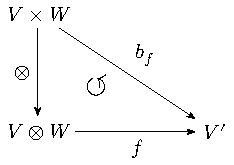
\includegraphics[width=0.3\linewidth]{tensor_product_diagram.pdf}
\end{minipage}
\bigbreak

\cref{thm:tensor-bijection}の証明には多くの予備知識が必要であるので省略する.




\subsection{線形写像のテンソル積}
\label{sec:tensor-product-of-linear-map}

$V, V', W, W'$をベクトル空間,
$f \colon V \to V'$,$g \colon W \to W'$を線形写像とする.
線形写像$f \otimes g \colon V \otimes W \to V' \otimes W'$を
\begin{equation}
    \label{eq:tensor-product-of-linear-map}
    (f \otimes g)(𝒙 \otimes 𝒚)
        = f(𝒙) \otimes g(𝒚)
\end{equation}
で定めたものを,$f$と$g$の\word{テンソル積}\index{てんそるせき@テンソル積}という%
\footnote{
    \cref{eq:tensor-product-of-linear-map}にある3つの$\otimes$はそれぞれ別の演算である.
    ひとつめは$\otimes \colon \hom(V, V') \times \hom(W, W') \to \hom ( V \otimes W, \  V' \otimes W' )$,
    ふたつめは$\otimes \colon V \times W \to V \otimes W$,
    みっつめは$\otimes \colon V' \times W' \to V' \otimes W'$である.
}.

\end{document}